% Options for packages loaded elsewhere
\PassOptionsToPackage{unicode}{hyperref}
\PassOptionsToPackage{hyphens}{url}
%
\documentclass[
]{article}
\usepackage{amsmath,amssymb}
\usepackage{lmodern}
\usepackage{iftex}
\ifPDFTeX
  \usepackage[T1]{fontenc}
  \usepackage[utf8]{inputenc}
  \usepackage{textcomp} % provide euro and other symbols
\else % if luatex or xetex
  \usepackage{unicode-math}
  \defaultfontfeatures{Scale=MatchLowercase}
  \defaultfontfeatures[\rmfamily]{Ligatures=TeX,Scale=1}
\fi
% Use upquote if available, for straight quotes in verbatim environments
\IfFileExists{upquote.sty}{\usepackage{upquote}}{}
\IfFileExists{microtype.sty}{% use microtype if available
  \usepackage[]{microtype}
  \UseMicrotypeSet[protrusion]{basicmath} % disable protrusion for tt fonts
}{}
\makeatletter
\@ifundefined{KOMAClassName}{% if non-KOMA class
  \IfFileExists{parskip.sty}{%
    \usepackage{parskip}
  }{% else
    \setlength{\parindent}{0pt}
    \setlength{\parskip}{6pt plus 2pt minus 1pt}}
}{% if KOMA class
  \KOMAoptions{parskip=half}}
\makeatother
\usepackage{xcolor}
\usepackage[margin=1in]{geometry}
\usepackage{color}
\usepackage{fancyvrb}
\newcommand{\VerbBar}{|}
\newcommand{\VERB}{\Verb[commandchars=\\\{\}]}
\DefineVerbatimEnvironment{Highlighting}{Verbatim}{commandchars=\\\{\}}
% Add ',fontsize=\small' for more characters per line
\usepackage{framed}
\definecolor{shadecolor}{RGB}{248,248,248}
\newenvironment{Shaded}{\begin{snugshade}}{\end{snugshade}}
\newcommand{\AlertTok}[1]{\textcolor[rgb]{0.94,0.16,0.16}{#1}}
\newcommand{\AnnotationTok}[1]{\textcolor[rgb]{0.56,0.35,0.01}{\textbf{\textit{#1}}}}
\newcommand{\AttributeTok}[1]{\textcolor[rgb]{0.77,0.63,0.00}{#1}}
\newcommand{\BaseNTok}[1]{\textcolor[rgb]{0.00,0.00,0.81}{#1}}
\newcommand{\BuiltInTok}[1]{#1}
\newcommand{\CharTok}[1]{\textcolor[rgb]{0.31,0.60,0.02}{#1}}
\newcommand{\CommentTok}[1]{\textcolor[rgb]{0.56,0.35,0.01}{\textit{#1}}}
\newcommand{\CommentVarTok}[1]{\textcolor[rgb]{0.56,0.35,0.01}{\textbf{\textit{#1}}}}
\newcommand{\ConstantTok}[1]{\textcolor[rgb]{0.00,0.00,0.00}{#1}}
\newcommand{\ControlFlowTok}[1]{\textcolor[rgb]{0.13,0.29,0.53}{\textbf{#1}}}
\newcommand{\DataTypeTok}[1]{\textcolor[rgb]{0.13,0.29,0.53}{#1}}
\newcommand{\DecValTok}[1]{\textcolor[rgb]{0.00,0.00,0.81}{#1}}
\newcommand{\DocumentationTok}[1]{\textcolor[rgb]{0.56,0.35,0.01}{\textbf{\textit{#1}}}}
\newcommand{\ErrorTok}[1]{\textcolor[rgb]{0.64,0.00,0.00}{\textbf{#1}}}
\newcommand{\ExtensionTok}[1]{#1}
\newcommand{\FloatTok}[1]{\textcolor[rgb]{0.00,0.00,0.81}{#1}}
\newcommand{\FunctionTok}[1]{\textcolor[rgb]{0.00,0.00,0.00}{#1}}
\newcommand{\ImportTok}[1]{#1}
\newcommand{\InformationTok}[1]{\textcolor[rgb]{0.56,0.35,0.01}{\textbf{\textit{#1}}}}
\newcommand{\KeywordTok}[1]{\textcolor[rgb]{0.13,0.29,0.53}{\textbf{#1}}}
\newcommand{\NormalTok}[1]{#1}
\newcommand{\OperatorTok}[1]{\textcolor[rgb]{0.81,0.36,0.00}{\textbf{#1}}}
\newcommand{\OtherTok}[1]{\textcolor[rgb]{0.56,0.35,0.01}{#1}}
\newcommand{\PreprocessorTok}[1]{\textcolor[rgb]{0.56,0.35,0.01}{\textit{#1}}}
\newcommand{\RegionMarkerTok}[1]{#1}
\newcommand{\SpecialCharTok}[1]{\textcolor[rgb]{0.00,0.00,0.00}{#1}}
\newcommand{\SpecialStringTok}[1]{\textcolor[rgb]{0.31,0.60,0.02}{#1}}
\newcommand{\StringTok}[1]{\textcolor[rgb]{0.31,0.60,0.02}{#1}}
\newcommand{\VariableTok}[1]{\textcolor[rgb]{0.00,0.00,0.00}{#1}}
\newcommand{\VerbatimStringTok}[1]{\textcolor[rgb]{0.31,0.60,0.02}{#1}}
\newcommand{\WarningTok}[1]{\textcolor[rgb]{0.56,0.35,0.01}{\textbf{\textit{#1}}}}
\usepackage{graphicx}
\makeatletter
\def\maxwidth{\ifdim\Gin@nat@width>\linewidth\linewidth\else\Gin@nat@width\fi}
\def\maxheight{\ifdim\Gin@nat@height>\textheight\textheight\else\Gin@nat@height\fi}
\makeatother
% Scale images if necessary, so that they will not overflow the page
% margins by default, and it is still possible to overwrite the defaults
% using explicit options in \includegraphics[width, height, ...]{}
\setkeys{Gin}{width=\maxwidth,height=\maxheight,keepaspectratio}
% Set default figure placement to htbp
\makeatletter
\def\fps@figure{htbp}
\makeatother
\setlength{\emergencystretch}{3em} % prevent overfull lines
\providecommand{\tightlist}{%
  \setlength{\itemsep}{0pt}\setlength{\parskip}{0pt}}
\setcounter{secnumdepth}{-\maxdimen} % remove section numbering
\ifLuaTeX
  \usepackage{selnolig}  % disable illegal ligatures
\fi
\IfFileExists{bookmark.sty}{\usepackage{bookmark}}{\usepackage{hyperref}}
\IfFileExists{xurl.sty}{\usepackage{xurl}}{} % add URL line breaks if available
\urlstyle{same} % disable monospaced font for URLs
\hypersetup{
  pdftitle={WORKING EXAMPLE 2},
  pdfauthor={Itziar Irigoien, Patricia Mas-Bermejo, Sergi Papiol, Neus Barrantes-Vidal,; Araceli Rosa, and Concepción Arenas},
  hidelinks,
  pdfcreator={LaTeX via pandoc}}

\title{WORKING EXAMPLE 2}
\usepackage{etoolbox}
\makeatletter
\providecommand{\subtitle}[1]{% add subtitle to \maketitle
  \apptocmd{\@title}{\par {\large #1 \par}}{}{}
}
\makeatother
\subtitle{In: A guide to test association between Polygenic Risk Scores
and psychological and psychiatric traits: practical examples}
\author{Itziar Irigoien, Patricia Mas-Bermejo, Sergi Papiol, Neus
Barrantes-Vidal, \and Araceli Rosa, and Concepción Arenas}
\date{}

\begin{document}
\maketitle

\hypertarget{working-flow-and-code}{%
\subsection{Working flow and code}\label{working-flow-and-code}}

In this example we simulate 10 PRSs, and a continuous trait, with sex,
clinical diagnosis (with 2 categories), age, and two Principal
Components as covariates.

\begin{itemize}
\tightlist
\item
  data reading
\end{itemize}

\begin{Shaded}
\begin{Highlighting}[]
\NormalTok{dat }\OtherTok{\textless{}{-}} \FunctionTok{read.table}\NormalTok{(}\StringTok{"WExample2.csv"}\NormalTok{, }\AttributeTok{header=}\ConstantTok{TRUE}\NormalTok{, }\AttributeTok{sep=}\StringTok{";"}\NormalTok{, }\AttributeTok{dec=}\StringTok{","}\NormalTok{)}
\FunctionTok{names}\NormalTok{(dat) }\CommentTok{\#}
\end{Highlighting}
\end{Shaded}

\begin{verbatim}
##  [1] "Diagnostic" "Sex"        "Age"        "Trait"      "PRS.1"     
##  [6] "PRS.2"      "PRS.3"      "PRS.4"      "PRS.5"      "PRS.6"     
## [11] "PRS.7"      "PRS.8"      "PRS.9"      "PRS.10"     "PC1"       
## [16] "PC2"
\end{verbatim}

\bigskip

\begin{itemize}
\tightlist
\item
  do not forget to declare the categorical variables as factors
\end{itemize}

\begin{Shaded}
\begin{Highlighting}[]
\NormalTok{dat}\SpecialCharTok{$}\NormalTok{Sex }\OtherTok{\textless{}{-}} \FunctionTok{as.factor}\NormalTok{(dat}\SpecialCharTok{$}\NormalTok{Sex)}
\NormalTok{dat}\SpecialCharTok{$}\NormalTok{Diagnostic }\OtherTok{\textless{}{-}} \FunctionTok{as.factor}\NormalTok{(dat}\SpecialCharTok{$}\NormalTok{Diagnostic)}
\end{Highlighting}
\end{Shaded}

\hypertarget{what-full-model-should-be-considered}{%
\subsection{1. What full model should be
considered?}\label{what-full-model-should-be-considered}}

\begin{itemize}
\tightlist
\item
  First, given a particular PRS (named PRS.i), consider all the possible
  full models:
\item
  FM\(_{WI}\): Trait versus PRS.i + Sex + Diagnostic + Age + PC1 + PC2
\item
  FM\(_{Sex}\): Trait versus PRS.i + Sex + PRS.i · Sex + Diagnostic +
  Age + PC1 + PC2
\item
  FM\(_{Diagnostic}\): Trait versus PRS.i + Sex + Diagnostic + PRS.i ·
  Diagnostic + Age + PC1 + PC2
\item
  FM\(_{Sex/Diagnostic}\): Trait versus PRS.i + Sex + PRS.i · Sex +
  Diagnostic + PRS.i · Diagnostic + Age + PC1 + PC2
\end{itemize}

\hypertarget{how-to-make-a-prs-ranking-to-find-the-important-ones}{%
\subsection{2. How to make a PRS ranking to find the important
ones?}\label{how-to-make-a-prs-ranking-to-find-the-important-ones}}

As is described in the paper, for each model, calculate the coefficient
of determination \(R^2\) and calculate the sum:
\(S = R^2_{WI} + R^2_{Sex} + R^2_{Diagnostic} + R^2_{Sex/Diagnostic}\).

According to S, list the PRSs in decreasing order.

\begin{Shaded}
\begin{Highlighting}[]
\NormalTok{out }\OtherTok{\textless{}{-}} \FunctionTok{orderR2}\NormalTok{(dat, }\AttributeTok{yname=}\StringTok{"Trait"}\NormalTok{, }\AttributeTok{prsname =} \StringTok{"PRS."}\NormalTok{)}
\FunctionTok{head}\NormalTok{(out)}
\end{Highlighting}
\end{Shaded}

\begin{verbatim}
##            Model1     Model2    Model3    Model4       Sum
## PRS.5  0.06590991 0.14386357 0.1167506 0.1730818 0.4996059
## PRS.10 0.04263225 0.05908320 0.1400714 0.1838914 0.4256782
## PRS.8  0.05330296 0.07034766 0.1239488 0.1626609 0.4102603
## PRS.2  0.06157642 0.06212837 0.1293514 0.1294614 0.3825176
## PRS.9  0.03691860 0.07445585 0.1061419 0.1443078 0.3618242
## PRS.1  0.06250443 0.06260526 0.1138417 0.1140869 0.3530384
\end{verbatim}

\begin{Shaded}
\begin{Highlighting}[]
\NormalTok{mainfilename }\OtherTok{\textless{}{-}} \StringTok{"WExample2"}
\NormalTok{filename }\OtherTok{\textless{}{-}} \FunctionTok{paste0}\NormalTok{(mainfilename, }\StringTok{"\_Ordered\_PRS.csv"}\NormalTok{)}
\FunctionTok{write.csv2}\NormalTok{(out,}\AttributeTok{file=}\NormalTok{filename)}
\end{Highlighting}
\end{Shaded}

\bigskip

Plot the sum of coefficients of determination \(S_{R^2}\). Lines: in
blue the median; in black the mean.

\begin{Shaded}
\begin{Highlighting}[]
\NormalTok{out }\OtherTok{\textless{}{-}} \FunctionTok{data.frame}\NormalTok{(out) }
\NormalTok{n }\OtherTok{\textless{}{-}} \FunctionTok{dim}\NormalTok{(out)[}\DecValTok{1}\NormalTok{]}
\NormalTok{select }\OtherTok{\textless{}{-}} \FunctionTok{grep}\NormalTok{(}\StringTok{"Model"}\NormalTok{, }\FunctionTok{names}\NormalTok{(out), }\AttributeTok{value=}\ConstantTok{FALSE}\NormalTok{)}
\NormalTok{out}\SpecialCharTok{$}\NormalTok{effect }\OtherTok{\textless{}{-}}\NormalTok{ out}\SpecialCharTok{$}\NormalTok{Sum}
\NormalTok{sds }\OtherTok{\textless{}{-}} \FunctionTok{apply}\NormalTok{(out[, select], }\DecValTok{1}\NormalTok{, sd)}
\NormalTok{out}\SpecialCharTok{$}\NormalTok{lower }\OtherTok{\textless{}{-}}\NormalTok{ out}\SpecialCharTok{$}\NormalTok{effect }\SpecialCharTok{{-}}\NormalTok{ sds}
\NormalTok{out}\SpecialCharTok{$}\NormalTok{upper }\OtherTok{\textless{}{-}}\NormalTok{ out}\SpecialCharTok{$}\NormalTok{effect }\SpecialCharTok{+}\NormalTok{ sds}
\NormalTok{out}\SpecialCharTok{$}\NormalTok{rank }\OtherTok{\textless{}{-}}\NormalTok{ n}\SpecialCharTok{:}\DecValTok{1}


\FunctionTok{ggplot}\NormalTok{(}\AttributeTok{data=}\NormalTok{out, }\FunctionTok{aes}\NormalTok{(}\AttributeTok{y=}\NormalTok{rank, }\AttributeTok{x=}\NormalTok{effect, }\AttributeTok{xmin=}\NormalTok{lower, }\AttributeTok{xmax=}\NormalTok{upper)) }\SpecialCharTok{+}
  \FunctionTok{geom\_point}\NormalTok{() }\SpecialCharTok{+}
  \FunctionTok{geom\_errorbarh}\NormalTok{(}\AttributeTok{height=}\NormalTok{.}\DecValTok{1}\NormalTok{) }\SpecialCharTok{+}
  \FunctionTok{scale\_y\_continuous}\NormalTok{(}\AttributeTok{name=}\ConstantTok{NULL}\NormalTok{, }\AttributeTok{breaks=}\NormalTok{ n}\SpecialCharTok{:}\DecValTok{1}\NormalTok{, }\AttributeTok{labels=}\FunctionTok{row.names}\NormalTok{(out), }\AttributeTok{position=}\StringTok{"right"}\NormalTok{) }\SpecialCharTok{+}
  \FunctionTok{labs}\NormalTok{(}\AttributeTok{title=}\StringTok{\textquotesingle{}\textquotesingle{}}\NormalTok{, }\AttributeTok{x=}\StringTok{\textquotesingle{}Sum R\^{}2\textquotesingle{}}\NormalTok{, }\AttributeTok{y =} \StringTok{\textquotesingle{}PRS\textquotesingle{}}\NormalTok{) }\SpecialCharTok{+}
  \FunctionTok{geom\_vline}\NormalTok{(}\AttributeTok{xintercept=}\FunctionTok{mean}\NormalTok{(out}\SpecialCharTok{$}\NormalTok{effect), }\AttributeTok{color=}\StringTok{\textquotesingle{}black\textquotesingle{}}\NormalTok{, }\AttributeTok{linetype=}\StringTok{\textquotesingle{}dashed\textquotesingle{}}\NormalTok{) }\SpecialCharTok{+}
  \FunctionTok{geom\_vline}\NormalTok{(}\AttributeTok{xintercept=}\FunctionTok{median}\NormalTok{(out}\SpecialCharTok{$}\NormalTok{effect), }\AttributeTok{color=}\StringTok{\textquotesingle{}blue\textquotesingle{}}\NormalTok{, }\AttributeTok{linetype=}\StringTok{\textquotesingle{}dashed\textquotesingle{}}\NormalTok{) }\SpecialCharTok{+}
  \FunctionTok{theme\_minimal}\NormalTok{()}
\end{Highlighting}
\end{Shaded}

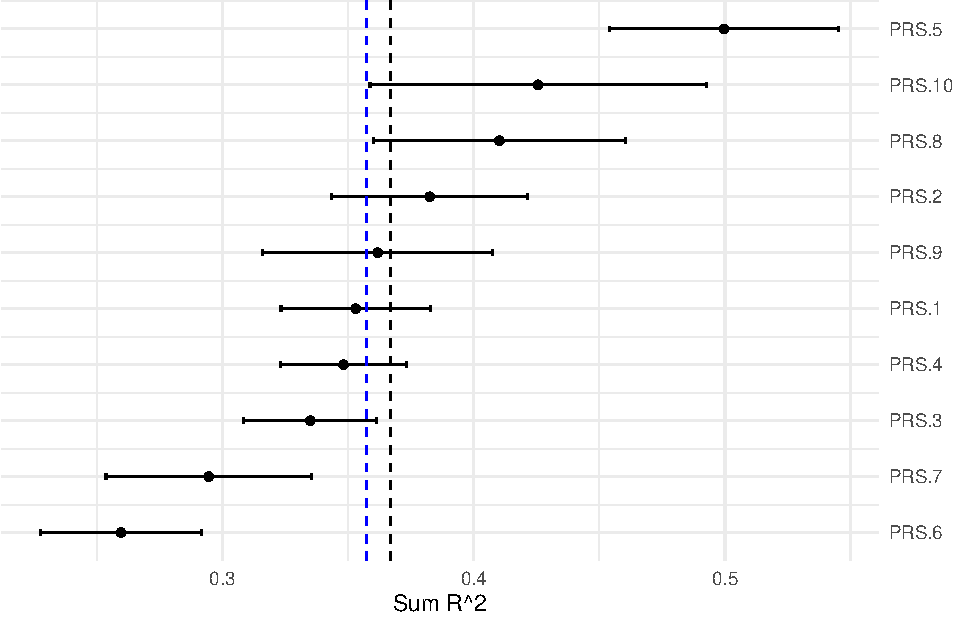
\includegraphics{WorkingExample2_code_files/figure-latex/unnamed-chunk-5-1.pdf}

According to the obtained results, first PRS.5 is selected to analyse
its association with the Trait.

\hypertarget{which-model-of-all-the-possible-ones-should-be-used}{%
\subsection{3. Which model, of all the possible ones, should be
used?}\label{which-model-of-all-the-possible-ones-should-be-used}}

The following figure represents the scatter plot of Trait versus PRS.5
separated by Sex and Diagnostic groups.

\begin{Shaded}
\begin{Highlighting}[]
\FunctionTok{ggplot}\NormalTok{(dat, }\FunctionTok{aes}\NormalTok{(}\AttributeTok{x=}\NormalTok{PRS}\FloatTok{.5}\NormalTok{, }\AttributeTok{y=}\NormalTok{Trait)) }\SpecialCharTok{+}
  \FunctionTok{geom\_point}\NormalTok{() }\SpecialCharTok{+}
  \FunctionTok{geom\_smooth}\NormalTok{(}\AttributeTok{method=}\NormalTok{lm, }\AttributeTok{se=}\ConstantTok{FALSE}\NormalTok{)}\SpecialCharTok{+}
  \FunctionTok{facet\_grid}\NormalTok{(Sex }\SpecialCharTok{\textasciitilde{}}\NormalTok{ Diagnostic, }\AttributeTok{labeller=}\NormalTok{label\_both)}
\end{Highlighting}
\end{Shaded}

\begin{verbatim}
## `geom_smooth()` using formula = 'y ~ x'
\end{verbatim}

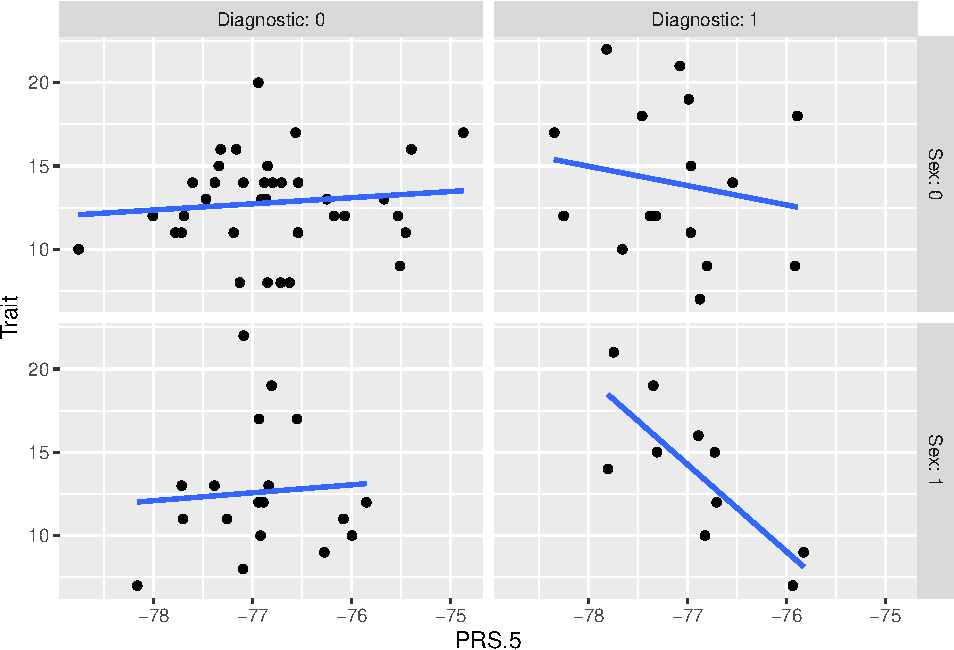
\includegraphics{WorkingExample2_code_files/figure-latex/unnamed-chunk-6-1.pdf}

\begin{Shaded}
\begin{Highlighting}[]
\CommentTok{\# Candidate FM Trait \textasciitilde{} PRS + Sex + Diagnostic + PRS + PRS*Diagnostic + PC1 +PC2}
\end{Highlighting}
\end{Shaded}

The plots suggest that the interaction between the PRS.5 and the
diagnostic is relevant. Thus, we set the full model candidate (FM):
\(Trait \sim PRS + Sex + Diagnostic + Sex + PRS \cdot Diagnostic + PC1 +PC2\).

\hypertarget{for-a-continuous-trait-what-steps-should-be-followed-for-a-correct-analysis}{%
\subsection{4. For a continuous trait, what steps should be followed for
a correct
analysis?}\label{for-a-continuous-trait-what-steps-should-be-followed-for-a-correct-analysis}}

\begin{itemize}
\tightlist
\item
  \textbf{4.1. How is the candidate model validated?}
\end{itemize}

First, we validate the normality of the errors and the constant variance
conditions (see the figures and the results of Shapiro test and Levene
test).

\begin{Shaded}
\begin{Highlighting}[]
\CommentTok{\#model}
\NormalTok{FM }\OtherTok{\textless{}{-}} \FunctionTok{lm}\NormalTok{(Trait }\SpecialCharTok{\textasciitilde{}}\NormalTok{ PRS}\FloatTok{.5}\SpecialCharTok{*}\NormalTok{Diagnostic }\SpecialCharTok{+}\NormalTok{ Sex }\SpecialCharTok{+}\NormalTok{ Age }\SpecialCharTok{+}\NormalTok{ PC1 }\SpecialCharTok{+}\NormalTok{ PC2, }\AttributeTok{data=}\NormalTok{dat)}
\CommentTok{\#qq{-}plot for normality }
\FunctionTok{plot}\NormalTok{(FM,}\DecValTok{2}\NormalTok{)   }
\end{Highlighting}
\end{Shaded}

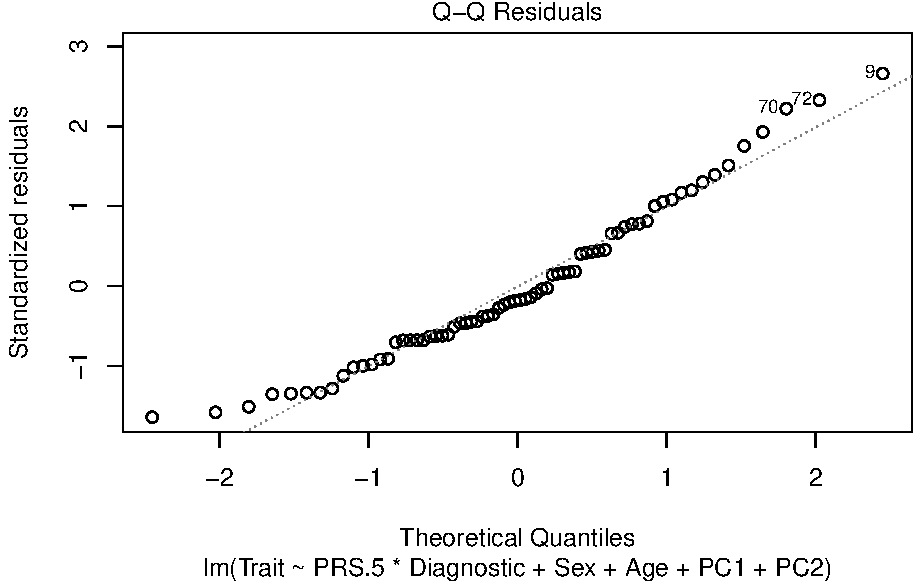
\includegraphics{WorkingExample2_code_files/figure-latex/unnamed-chunk-7-1.pdf}

Lack of normality of residuals is suggested and this is supported by
Shapiro's test.

\begin{Shaded}
\begin{Highlighting}[]
\CommentTok{\#Shapiro{-}Wilk test}
\FunctionTok{shapiro.test}\NormalTok{(FM}\SpecialCharTok{$}\NormalTok{residuals)}
\end{Highlighting}
\end{Shaded}

\begin{verbatim}
## 
##  Shapiro-Wilk normality test
## 
## data:  FM$residuals
## W = 0.96257, p-value = 0.03475
\end{verbatim}

\begin{Shaded}
\begin{Highlighting}[]
\CommentTok{\#plot for variances}
\NormalTok{d }\OtherTok{\textless{}{-}} \FunctionTok{fortify}\NormalTok{(FM)}
\FunctionTok{ggplot}\NormalTok{(d,}\FunctionTok{aes}\NormalTok{(}\AttributeTok{x=}\NormalTok{.fitted, }\AttributeTok{y=}\NormalTok{.stdresid, }\AttributeTok{colour=}\NormalTok{Diagnostic)) }\SpecialCharTok{+} 
  \FunctionTok{geom\_point}\NormalTok{() }\SpecialCharTok{+} 
  \FunctionTok{geom\_hline}\NormalTok{(}\AttributeTok{yintercept=}\DecValTok{0}\NormalTok{, }\AttributeTok{col=}\StringTok{"red"}\NormalTok{)}\SpecialCharTok{+}
  \FunctionTok{facet\_wrap}\NormalTok{(.}\SpecialCharTok{\textasciitilde{}}\NormalTok{Diagnostic)}
\end{Highlighting}
\end{Shaded}

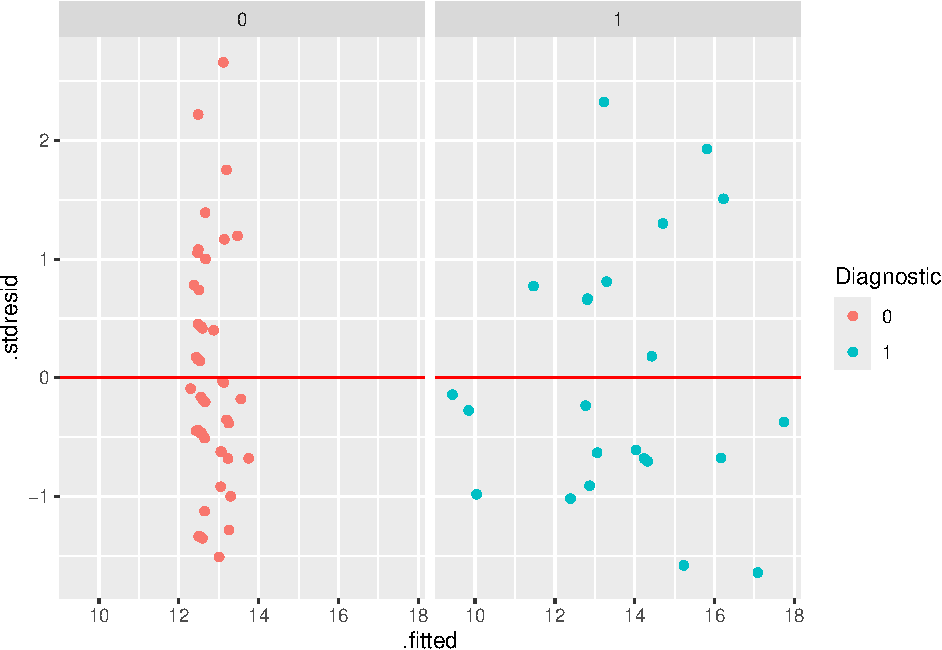
\includegraphics{WorkingExample2_code_files/figure-latex/unnamed-chunk-9-1.pdf}

\begin{Shaded}
\begin{Highlighting}[]
\CommentTok{\#Levene\textquotesingle{}s test}
\FunctionTok{leveneTest}\NormalTok{(.stdresid }\SpecialCharTok{\textasciitilde{}}\NormalTok{ Diagnostic, }\AttributeTok{data=}\NormalTok{d)}
\end{Highlighting}
\end{Shaded}

\begin{verbatim}
## Levene's Test for Homogeneity of Variance (center = median)
##       Df F value Pr(>F)
## group  1  0.4042 0.5271
##       68
\end{verbatim}

The figure does not show problems with the residuals, although it can be
seen that for Diagnostic group 1 their variability increases as the
fitted values do so, suggesting possible problems with the homogeneity
of variances. However, Levene's test does not indicate evidence against
homoscedasticity, neither a trend is observed that could indicate a lack
of linearity.

\begin{itemize}
\tightlist
\item
  \textbf{4.2. What can be done if any validation condition fails?}
\end{itemize}

We have two approaches to assess the possible association with PRS.5 and
the Trait: try a transformation of the trait or perform a permutation
test.

First, we try a transformation. Given the shape of the density of
residuals given by the next figure, the logarithmic transformation seems
adequate to achieve normality.

\begin{Shaded}
\begin{Highlighting}[]
\CommentTok{\#Histogram of the residuals}
\FunctionTok{hist}\NormalTok{(FM}\SpecialCharTok{$}\NormalTok{residuals)}
\end{Highlighting}
\end{Shaded}

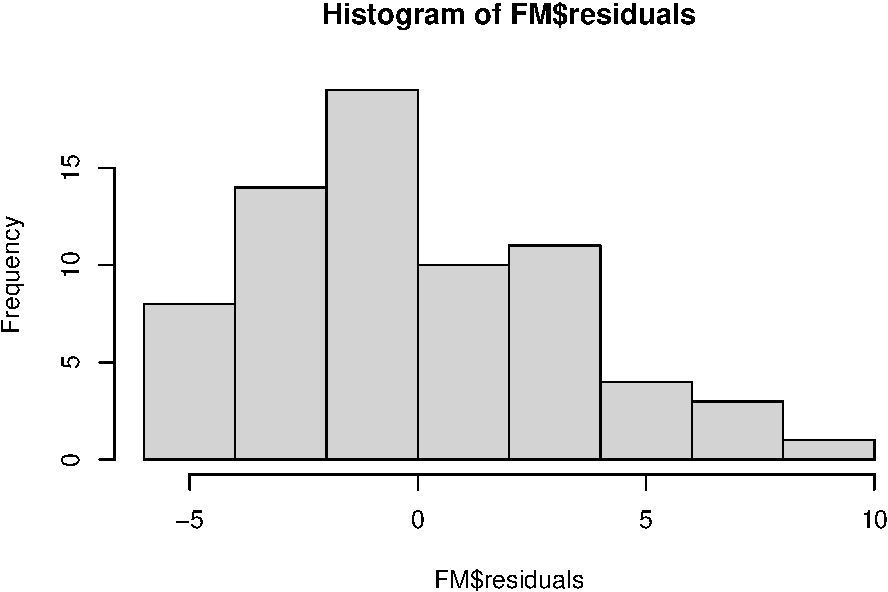
\includegraphics{WorkingExample2_code_files/figure-latex/unnamed-chunk-11-1.pdf}

\begin{Shaded}
\begin{Highlighting}[]
\NormalTok{dat}\SpecialCharTok{$}\NormalTok{logTrait }\OtherTok{\textless{}{-}} \FunctionTok{log}\NormalTok{(dat}\SpecialCharTok{$}\NormalTok{Trait)}
\NormalTok{FM }\OtherTok{\textless{}{-}} \FunctionTok{lm}\NormalTok{(logTrait }\SpecialCharTok{\textasciitilde{}}\NormalTok{ PRS}\FloatTok{.5}\SpecialCharTok{*}\NormalTok{Diagnostic }\SpecialCharTok{+}\NormalTok{ Sex }\SpecialCharTok{+}\NormalTok{ Age }\SpecialCharTok{+}\NormalTok{ PC1 }\SpecialCharTok{+}\NormalTok{ PC2, }\AttributeTok{data=}\NormalTok{dat)}
\CommentTok{\#qq{-}plot for normality }
\FunctionTok{plot}\NormalTok{(FM,}\DecValTok{2}\NormalTok{)}
\end{Highlighting}
\end{Shaded}

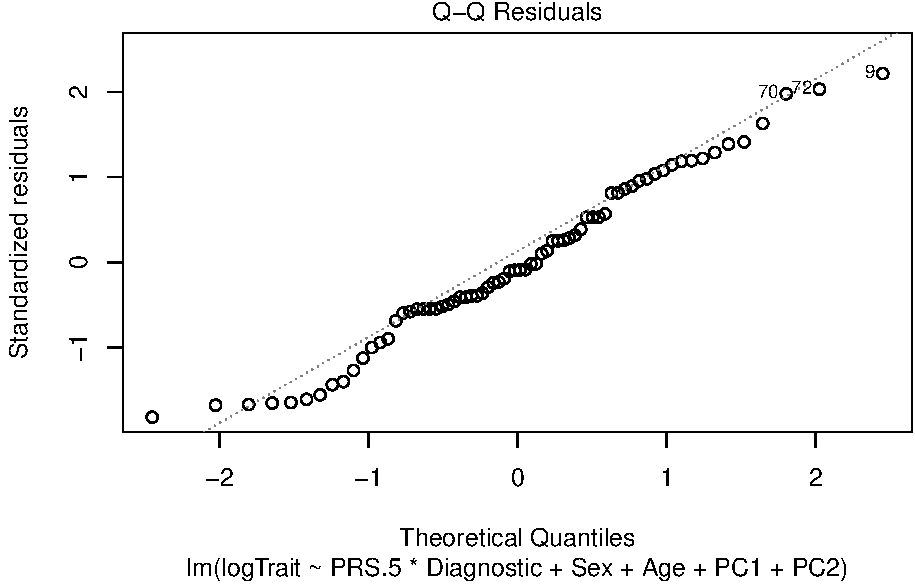
\includegraphics{WorkingExample2_code_files/figure-latex/unnamed-chunk-12-1.pdf}

\begin{Shaded}
\begin{Highlighting}[]
\CommentTok{\#Shapiro{-}Wilk test}
\FunctionTok{shapiro.test}\NormalTok{(FM}\SpecialCharTok{$}\NormalTok{residuals)}
\end{Highlighting}
\end{Shaded}

\begin{verbatim}
## 
##  Shapiro-Wilk normality test
## 
## data:  FM$residuals
## W = 0.97729, p-value = 0.2331
\end{verbatim}

Thus, it is suggested the transformation offered a solution for the lack
of normality. Furthermore,

\begin{Shaded}
\begin{Highlighting}[]
\CommentTok{\#plot for variances}
\NormalTok{d }\OtherTok{\textless{}{-}} \FunctionTok{fortify}\NormalTok{(FM)}
\FunctionTok{ggplot}\NormalTok{(d,}\FunctionTok{aes}\NormalTok{(}\AttributeTok{x=}\NormalTok{.fitted, }\AttributeTok{y=}\NormalTok{.stdresid, }\AttributeTok{colour=}\NormalTok{Diagnostic)) }\SpecialCharTok{+} 
  \FunctionTok{geom\_point}\NormalTok{() }\SpecialCharTok{+} 
  \FunctionTok{geom\_hline}\NormalTok{(}\AttributeTok{yintercept=}\DecValTok{0}\NormalTok{, }\AttributeTok{col=}\StringTok{"red"}\NormalTok{)}\SpecialCharTok{+}
  \FunctionTok{facet\_wrap}\NormalTok{(.}\SpecialCharTok{\textasciitilde{}}\NormalTok{Diagnostic)}
\end{Highlighting}
\end{Shaded}

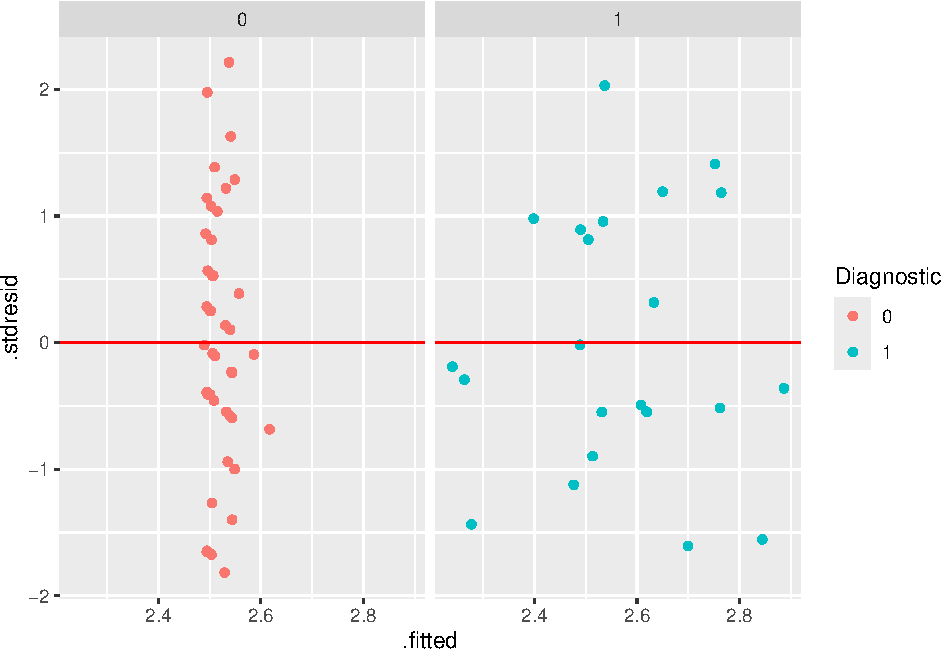
\includegraphics{WorkingExample2_code_files/figure-latex/unnamed-chunk-14-1.pdf}

\begin{Shaded}
\begin{Highlighting}[]
\CommentTok{\#Levene\textquotesingle{}s test}
\FunctionTok{leveneTest}\NormalTok{(.stdresid }\SpecialCharTok{\textasciitilde{}}\NormalTok{ Diagnostic, }\AttributeTok{data=}\NormalTok{d)}
\end{Highlighting}
\end{Shaded}

\begin{verbatim}
## Levene's Test for Homogeneity of Variance (center = median)
##       Df F value Pr(>F)
## group  1  0.1157 0.7348
##       68
\end{verbatim}

it does not indicate evidence against homoscedasticity, neither a trend
is observed that could indicate a lack of linearity.

Then, the model we build is given by:

\begin{Shaded}
\begin{Highlighting}[]
\FunctionTok{summary}\NormalTok{(FM)}
\end{Highlighting}
\end{Shaded}

\begin{verbatim}
## 
## Call:
## lm(formula = logTrait ~ PRS.5 * Diagnostic + Sex + Age + PC1 + 
##     PC2, data = dat)
## 
## Residuals:
##      Min       1Q   Median       3Q      Max 
## -0.44983 -0.13453 -0.02147  0.20389  0.55307 
## 
## Coefficients:
##                     Estimate Std. Error t value Pr(>|t|)  
## (Intercept)        2.585e+00  4.118e+00   0.628   0.5325  
## PRS.5              8.892e-04  5.365e-02   0.017   0.9868  
## Diagnostic1       -2.005e+01  8.027e+00  -2.498   0.0152 *
## Sex1               4.141e-02  6.937e-02   0.597   0.5527  
## Age               -6.155e-04  6.528e-03  -0.094   0.9252  
## PC1                1.971e-01  4.669e-01   0.422   0.6744  
## PC2               -5.958e-02  4.440e-01  -0.134   0.8937  
## PRS.5:Diagnostic1 -2.607e-01  1.042e-01  -2.502   0.0150 *
## ---
## Signif. codes:  0 '***' 0.001 '**' 0.01 '*' 0.05 '.' 0.1 ' ' 1
## 
## Residual standard error: 0.2581 on 62 degrees of freedom
##   (11 observations deleted due to missingness)
## Multiple R-squared:  0.1518, Adjusted R-squared:  0.05609 
## F-statistic: 1.586 on 7 and 62 DF,  p-value: 0.1564
\end{verbatim}

The results show that PRS.5 is related with the log(Trait) in the
following way:

\begin{itemize}
\tightlist
\item
  \(\widehat{log(Trait)} = 2.585 + 0.00089\times PRS.5 + 0.041\times Sex - 0.0006\times Age + 0.197\times PC1 - 0.0596\times PC2\),
  if Diagnostic = 0;
\item
  \(\widehat{log(Trait)} = (2.585-20.052) + (0.00089-0.26068)\times PRS.5 + 0.041\times Sex + - 0.0006\times Age + 0.197\times PC1 - 0.0596\times PC2\),
  if Diagnostic = 1;
\end{itemize}

where Sex takes values 0 or 1, depending on whether the individual under
study is male or female, affecting only the value of the intercept.

If the objective is to evaluate the possible association between Trait
and PRS.5, it can be interesting to check whether the respective PRS.4
coefficients under each Diagnostic group are considerable or not.

\begin{Shaded}
\begin{Highlighting}[]
\FunctionTok{summary}\NormalTok{(}\FunctionTok{glht}\NormalTok{(FM, }\StringTok{"PRS.5 = 0"}\NormalTok{))}
\end{Highlighting}
\end{Shaded}

\begin{verbatim}
## 
##   Simultaneous Tests for General Linear Hypotheses
## 
## Fit: lm(formula = logTrait ~ PRS.5 * Diagnostic + Sex + Age + PC1 + 
##     PC2, data = dat)
## 
## Linear Hypotheses:
##             Estimate Std. Error t value Pr(>|t|)
## PRS.5 == 0 0.0008892  0.0536465   0.017    0.987
## (Adjusted p values reported -- single-step method)
\end{verbatim}

\begin{Shaded}
\begin{Highlighting}[]
\FunctionTok{summary}\NormalTok{(}\FunctionTok{glht}\NormalTok{(FM, }\StringTok{"PRS.5  + PRS.5:Diagnostic1 = 0"}\NormalTok{))}
\end{Highlighting}
\end{Shaded}

\begin{verbatim}
## 
##   Simultaneous Tests for General Linear Hypotheses
## 
## Fit: lm(formula = logTrait ~ PRS.5 * Diagnostic + Sex + Age + PC1 + 
##     PC2, data = dat)
## 
## Linear Hypotheses:
##                                Estimate Std. Error t value Pr(>|t|)   
## PRS.5 + PRS.5:Diagnostic1 == 0 -0.25979    0.08808  -2.949  0.00449 **
## ---
## Signif. codes:  0 '***' 0.001 '**' 0.01 '*' 0.05 '.' 0.1 ' ' 1
## (Adjusted p values reported -- single-step method)
\end{verbatim}

This means that for Diagnostic 1 the association is significant
(\(p\)-value= 0.004487) and negative and if PRS increases in one unit
while keeping the other predictors constant, the change in the Trait is
obtained multiplying by coeff = \(\exp(-0.25979)\) = 0.771; therefore it
will decrease. For Diagnostic 0 there is no significant association, and
if PRS increases in one unit while keeping the other predictors
constant, the expected change in the Trait is obtained multiplying by
coeff = exp(0.00089) = 1.001; thus no change is expected. The ratio
\(\widehat{log(Trait)}|_{PRS.5 = 1}/\widehat{log(Trait)}|_{PRS.5=0} = \exp(-0.25979)=0.771 < 1\),
thus, gives a mean decrease of about 22.9\%, for any given value (PRS.5=
prs value).

\bigskip

On the other hand, with the permutation approach:

\begin{Shaded}
\begin{Highlighting}[]
\NormalTok{NM }\OtherTok{\textless{}{-}} \FunctionTok{lm}\NormalTok{(Trait }\SpecialCharTok{\textasciitilde{}}\NormalTok{ Diagnostic }\SpecialCharTok{+}\NormalTok{ Sex }\SpecialCharTok{+}\NormalTok{ Age }\SpecialCharTok{+}\NormalTok{ PC1 }\SpecialCharTok{+}\NormalTok{ PC2, }\AttributeTok{data=}\NormalTok{dat)}
\NormalTok{FM }\OtherTok{\textless{}{-}} \FunctionTok{lm}\NormalTok{(Trait }\SpecialCharTok{\textasciitilde{}}\NormalTok{ PRS}\FloatTok{.5}\SpecialCharTok{*}\NormalTok{Diagnostic }\SpecialCharTok{+}\NormalTok{ Sex }\SpecialCharTok{+}\NormalTok{ Age }\SpecialCharTok{+}\NormalTok{ PC1 }\SpecialCharTok{+}\NormalTok{ PC2, }\AttributeTok{data=}\NormalTok{dat)}
\NormalTok{outperm }\OtherTok{\textless{}{-}} \FunctionTok{dR2}\NormalTok{(}\AttributeTok{NullModel=}\NormalTok{NM, }\AttributeTok{FullModel=}\NormalTok{FM, }\AttributeTok{B=}\DecValTok{1000}\NormalTok{, }\AttributeTok{seed=}\DecValTok{165}\NormalTok{)}
\NormalTok{outperm}
\end{Highlighting}
\end{Shaded}

\begin{verbatim}
## $dR2
## [1] 0.1078214
## 
## $pvalue
## [1] 0.014
\end{verbatim}

We observe an increase of 0.108 in the coefficient of determination when
the PRS.5 is included in the model and the permutation test indicates it
is significant.

\begin{itemize}
\tightlist
\item
  \textbf{Last step: We move to the next PRS.}
\end{itemize}

\end{document}
